\documentclass[12pt]{article}

\usepackage[margin=1in]{geometry}
\usepackage{graphicx}
\usepackage{booktabs}
\usepackage{longtable}
\usepackage{array}
\usepackage{listings}
\usepackage{xcolor}
\usepackage{hyperref}
\usepackage{caption}
\usepackage{setspace}

\hypersetup{
    colorlinks=true,
    linkcolor=black,
    urlcolor=blue
}

\lstset{
    basicstyle=\ttfamily\small,
    breaklines=true,
    frame=single,
    columns=fullflexible,
    keepspaces=true,
    showstringspaces=false,
    tabsize=4
}

\title{CSE 565 Structural-Based Testing Project}
\author{Chase Coleman}
\date{\today}

\begin{document}

\begin{titlepage}
    \centering
    \vspace*{1.5in}
    {\Large CSE 565 Structural-Based Testing Project\par}
    \vspace{0.75in}
    Chase Coleman\par
    Arizona State University\par
    CSE 565: Software Verification and Validation\par
    \vspace{0.75in}
    \today\par
\end{titlepage}

\setcounter{page}{2}
\doublespacing

\section{Introduction}

This report presents the results of a structural-based testing assignment. Part 1 uses test cases for the provided \texttt{VendingMachine.java} program and discusses statement and decision coverage. Part 2 uses PMD to perform static source code analysis on \texttt{StaticAnalysis.java} and evaluates the anomalies detected by the tool.

\section{Part 1: Vending Machine Testing}

\subsection{Tool Used and Coverage Type}

For Part 1, JUnit 5 and JaCoCo were used to test and measure coverage for \texttt{VendingMachine.java}. JUnit 5 provides the assertion framework used to execute each test case and compare the actual output from \texttt{dispenseItem} against the expected output (JUnit Team, n.d.). JaCoCo is a Java code coverage tool that instruments the compiled program during test execution and produces coverage reports after the tests finish (JaCoCo Team, n.d.).

JaCoCo reports several coverage measurements, including instruction coverage, line coverage, branch coverage, complexity coverage, method coverage, and class coverage (JaCoCo Team, n.d.). For this assignment, line coverage is used as the practical measurement for statement coverage because it shows whether the executable lines of the program were run. Branch coverage is used as the practical measurement for decision coverage because it shows whether the true and false outcomes of conditional decisions were exercised.

The tests and coverage report were run with Maven, a Java build tool that manages project compilation, testing, and documentation through a project object model file (Apache Software Foundation, n.d.), using the following command:

\begin{lstlisting}[language=bash,caption={JUnit and JaCoCo Test Command}]
mvn clean verify
\end{lstlisting}

\subsection{Test Cases Developed}

The test cases were selected to cover object construction, the available products, successful purchases, exact purchases, and insufficient-money cases. Table~\ref{tab:testcases} summarizes the cases.

\begin{longtable}{>{\raggedright\arraybackslash}p{1.6in}p{0.65in}p{0.75in}>{\raggedright\arraybackslash}p{2.8in}}
\caption{Vending Machine Test Cases}
\label{tab:testcases}\\
\toprule
Test & Input & Item & Expected Result \\
\midrule
\endfirsthead
\toprule
Test & Input & Item & Expected Result \\
\midrule
\endhead
Construct vending machine & N/A & N/A & A \texttt{VendingMachine} object is created successfully \\
Candy with extra money & 30 & candy & Item dispensed and change of 10 returned \\
Coke exact money & 25 & coke & Item dispensed. \\
Coffee exact money & 45 & coffee & Item dispensed. \\
Coffee, enough for candy or coke & 30 & coffee & Item not dispensed, missing 15 cents. Can purchase candy or coke. \\
Coffee, enough for candy only & 22 & coffee & Item not dispensed, missing 23 cents. Can purchase candy. \\
Coffee, not enough for anything & 10 & coffee & Item not dispensed, missing 35 cents. Cannot purchase item. \\
\bottomrule
\end{longtable}

\subsection{JUnit Test Code}

The following JUnit test code was written to execute the test cases. Each test uses assertions to confirm that the actual output from \texttt{dispenseItem} matches the expected result.

\lstinputlisting[language=Java,caption={Vending Machine JUnit Tests}]{src/test/java/VendingMachineTest.java}

\subsection{Test Execution Result}

The Maven test execution showed that all seven JUnit tests passed with no failures, errors, or skipped tests:

\begin{lstlisting}[caption={JUnit Test Execution Summary}]
Tests run: 7, Failures: 0, Errors: 0, Skipped: 0
All coverage checks have been met.
BUILD SUCCESS
\end{lstlisting}

Figure~\ref{fig:output} shows the JUnit test execution output. The final JUnit test suite contains seven tests, including one construction test so that JaCoCo records coverage for the implicit constructor line in \texttt{VendingMachine.java}.

\begin{figure}[h]
    \centering
    \IfFileExists{screenshots/test_execution.png}{
        \includegraphics[width=0.95\textwidth]{screenshots/test_execution.png}
    }{
        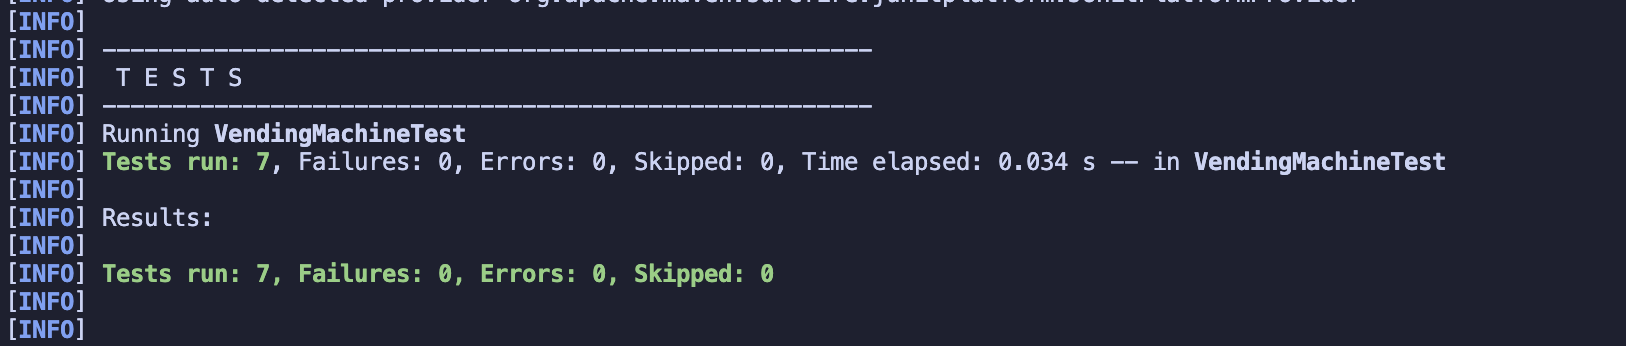
\includegraphics[width=0.95\textwidth]{screenshots/output.png}
    }
    \caption{JUnit test execution output for the vending machine}
    \label{fig:output}
\end{figure}

\subsection{Coverage Discussion}

The test suite was designed to exercise the main control-flow paths in \texttt{dispenseItem}. The construction test covers the class's implicit default constructor, which JaCoCo reports as an executable line. The product tests cover the product selection statements for candy, coke, and coffee. The successful-purchase tests cover the \texttt{input > cost} and \texttt{input == cost} branches. The remaining three tests cover the insufficient-money branch and the nested decisions for \texttt{input < 45}, \texttt{input < 25}, and \texttt{input < 20}.

Together, these tests execute the statements that assign product costs, compute change, assign successful return messages, assign insufficient-money messages, and return the final result. The insufficient-money tests were intentionally chosen at 30, 22, and 10 cents so that the nested decision logic is exercised across its different outcomes.

The JaCoCo report showed 0 missed lines and 24 covered lines, giving 100\% line coverage. It also showed 1 missed branch and 15 covered branches, giving 93.75\% branch coverage. This satisfies the assignment goals of 100\% statement coverage and at least 90\% decision coverage.

The only missed branch is the false outcome of \texttt{if(input < 45)} inside the insufficient-funds block. For the valid product inputs, this false branch is unreachable. The insufficient-funds block only executes when \texttt{input < cost}, and the highest valid product cost is coffee at 45 cents. Therefore, when the insufficient-funds block is reached for coffee, \texttt{input} must already be less than 45.

One implementation issue is that the vending machine code compares strings using \texttt{==}. These tests use Java string literals such as \texttt{"candy"}, \texttt{"coke"}, and \texttt{"coffee"}, so the current implementation behaves as expected because string literals are interned. In production code, \texttt{.equals()} would be safer because \texttt{==} compares object references rather than string contents.

\subsection{Coverage Report}

The JaCoCo CSV report generated by the test run is shown below. The report shows that \texttt{VendingMachine} achieved 100\% line coverage and 93.75\% branch coverage.

\lstinputlisting[caption={JaCoCo Coverage Summary}]{target/site/jacoco/jacoco.csv}

\IfFileExists{screenshots/coverage.png}{
    Figure~\ref{fig:coverage} shows the code coverage output achieved by the vending machine test cases.

    \begin{figure}[h]
        \centering
        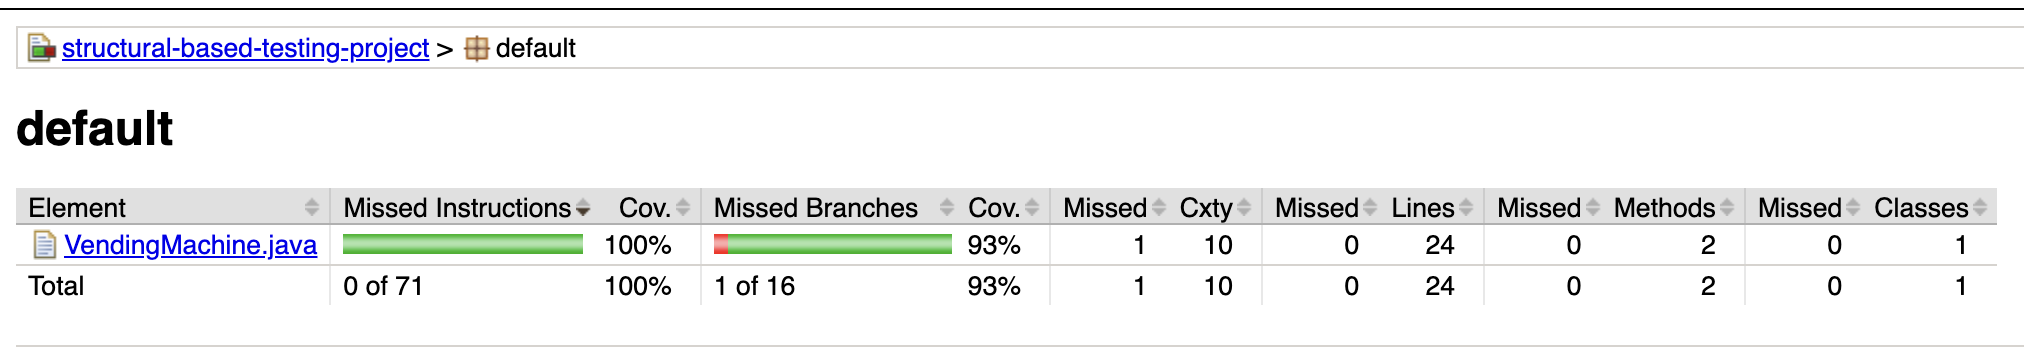
\includegraphics[width=0.95\textwidth]{screenshots/coverage.png}
        \caption{Vending machine code coverage result}
        \label{fig:coverage}
    \end{figure}
}{
    The JaCoCo HTML report is generated at \texttt{target/site/jacoco/index.html}. A screenshot of that page can be saved as \texttt{screenshots/coverage.png}; the report will include the screenshot automatically when the PDF is rebuilt.
}

\section{Part 2: Static Analysis}

\subsection{Tool Used and Analysis Type}

PMD 6.55.0 was used as the static source code analysis tool. PMD analyzes source code without executing the program. It can detect unused variables, questionable object comparisons, style issues, design issues, empty code blocks, duplicated code, overly complex methods, and other maintainability problems. For Java programs, PMD performs parsing, symbol resolution, and type resolution before rules inspect the source code (PMD Project, n.d.).

PMD was downloaded as a standalone distribution and run from the command line. The command used was:

\begin{lstlisting}[language=bash,caption={PMD Command}]
/tmp/pmd-bin-6.55.0/bin/run.sh pmd -d StaticAnalysis.java -R rulesets/java/quickstart.xml -f text > pmd_static_analysis_report.txt
\end{lstlisting}

\subsection{PMD Report}

The PMD report generated for \texttt{StaticAnalysis.java} is shown below.

\lstinputlisting[caption={PMD Static Analysis Report}]{pmd_static_analysis_report.txt}

\subsection{Anomalies Detected}

PMD detected unused local variables in the constructor on lines 15 and 16:

\begin{lstlisting}[language=Java]
int weight = 0;
String length = "";
\end{lstlisting}

These variables are assigned values but are never used. This is a data flow anomaly because the variables are defined without any later use.

PMD also detected a string comparison problem on line 24:

\begin{lstlisting}[language=Java]
if(product == "Electronics")
\end{lstlisting}

This is risky because Java's \texttt{==} operator compares object references. String contents should normally be compared with \texttt{.equals()}, such as:

\begin{lstlisting}[language=Java]
if ("Electronics".equals(product))
\end{lstlisting}

PMD also reported additional style and design findings, including no package declaration, a utility-class recommendation, and missing braces around control statements. These findings are useful, but the unused-variable and string-comparison findings are the most relevant anomalies for this assignment.

\subsection{Assessment of PMD}

PMD was effective for this assignment because it identified the major suspicious patterns in \texttt{StaticAnalysis.java}. The report included the line number, rule name, and a short description for each finding, which made the results easy to interpret.

The main features of PMD include command-line analysis, configurable rulesets, multiple output formats, and Java quality rules for correctness, maintainability, and style. PMD covers anomalies such as unused variables, questionable comparisons, empty statements, unnecessary code, and design problems.

The tool was easy to use because it required only a source file, a ruleset, and an output format. The main limitation is that PMD reports both important anomalies and minor style issues, so the user must interpret which findings are most relevant to the assignment.

\section{Conclusion}

The vending machine test cases exercise the main statement and decision paths in the provided program. The PMD static analysis identified the important anomalies in \texttt{StaticAnalysis.java}, especially unused variables and unsafe string comparison. Together, the two parts demonstrate both dynamic testing through executed test cases and static analysis through source code inspection.

\section*{References}

\hangindent=0.5in Apache Software Foundation. (n.d.). \textit{Welcome to Apache Maven}. Retrieved August 29, 2026, from \url{https://maven.apache.org/}

\hangindent=0.5in JaCoCo Team. (n.d.). \textit{JaCoCo Maven plug-in}. Retrieved August 29, 2026, from \url{https://www.jacoco.org/jacoco/trunk/doc/maven.html}

\hangindent=0.5in JUnit Team. (n.d.). \textit{JUnit 5 user guide}. Retrieved August 29, 2026, from \url{https://junit.org/junit5/docs/5.12.0/user-guide/index.html}

\hangindent=0.5in PMD Project. (n.d.). \textit{Java support}. Retrieved August 29, 2026, from \url{https://pmd.github.io/pmd/pmd_languages_java.html}

\end{document}
